In order to help practice applying PoLP in cloud projects, we have designed a Least Privilege CTF: a set of ``capture-the-flag'' exercises in which
players attempt to reduce the privileges of a policy attached to a member using the different processes described in Section~\ref{sec:gcpiam}.

\subsection{Design Goals}
To effectively teach developers about how to use IAM mechanisms to reduce privileges on Google Cloud Platform, the CTF has been designed
with several goals in mind.  These goals include:
\begin{itemize}
\item {\em Scaffolded}: Each level should incrementally build on prior levels in order to support consistent player progression.
\item {\em Differentiated instruction}: Exercises should provide explicit and detailed instructions that enable those familiar with IAM and those who are novices to complete.  Goals for each level and level gameplay should be consistent in order to ensure players focus on the specific concepts and skills being targeted.
\item {\em Immediate feedback}: Players should be able to receive results on their progress in each level as soon as possible as well as be given reasons why solution attempts might be failing.
\item {\em Easily deployed}: Exercises should be easy to deploy and at minimal cost the player.
\item {\em Extensible}: Additional exercises should be easily added to follow the evolution of the security mechanisms supported by IAM.
%% Minimum cost: Anyone can apply for 300 credits(dollars) for free with a Google account and credit card. If levels are deleted upon completion, monthly cost would be less than a dollar (Figure~\ref{fig:cost}). 
%% Fast Deployment:  Deploy initial 11 levels in 4.5 minutes.
\end{itemize}

\subsection{Implementation}
To meet the design goals, the Least Privilege CTF has been implemented with several key features.  These features include ...<FMI>

\subsubsection{Scaffolded conceptual progression}
Perhaps the most important aspect of an exercise is the progression of levels that players go through.  Towards this end, the CTF follows the progression
of concepts outlined in Section~\ref{sec:gcpiam}.  Initial levels expose players to the coarse, project-level, primitive roles that are often used in Quickstart
walkthroughs for convenience, but are often overprovisioned.  Players then progress to a variety of levels that show them how pre-defined roles can be used
to reduce the privileges from primitive roles.   Finally, players are then asked to create custom roles to generate an exact set of permissions that are
required for a particular access pattern.
Specifically, there are currently 11 levels in the Least Privilege CTF.  The levels are designed in a scaffolded style with incrementally increasing difficulties. 
-> project level primitive roles, 
Players may spend a little bit more time on the levels regarding Cloud Vision service - a service that does not have a set of predefined roles or permissions associated in GCP, indicating that the authenticated service accounts will have default access to Cloud Vision API. In order to analyse images with Cloud Vision service, the players are required to upload images into a Bucket through the form in front-end page (access function). The analysed results will be inserted into Cloud Datastore and listed in the same page.  The roles or permissions to complete such tasks are actually in Cloud Storage and Datastore category. The correct answer of level CustomRole-Vision is a combination of predefined role and custom role. As mentioned in Section~\ref{sec:gcpiam}, GCP does not support Datastore permissions in Custom Role yet.


In the design of Least Privilege CTF, all functions are expected to access level resources only with their default identities, the service accounts created and attached during deployment. The roles bind with these service accounts can be updated after deployment in Google Cloud Console. 
A check function validates whether the binding role(s) in access function matche(s) the correct answer, so a role with permissions to list and get roles or IAM policy is always required. The score board function is using similar technique to validate answers and calculate scores, and repeat this for all levels. The roles bind with access functions are more complicated and vary based on specific levels. In general, access functions begin with a role of excessive permissions to perform certain actions described in level instruction. The winning condition is to apply PoLP and grant minimum privileges that are just enough to perform the same action. The process of picking and specifying more restrictive roles has been exemplified in Section~\ref{sec:gcpiam}.

\subsubsection{Ease of gameplay}
\begin{figure}[!h]
  \centering
  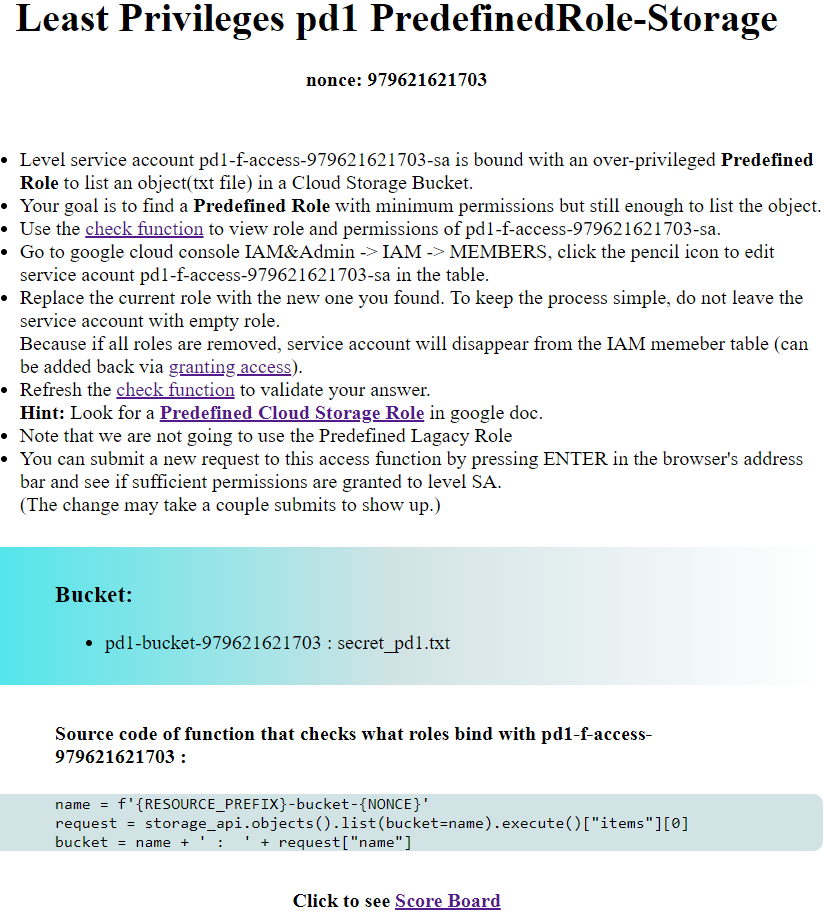
\includegraphics[width=0.5\textwidth]{pic/access}
  \caption {Access Function}
  \label{fig:access}
\end{figure}
\begin{figure}[!h]
  \centering
  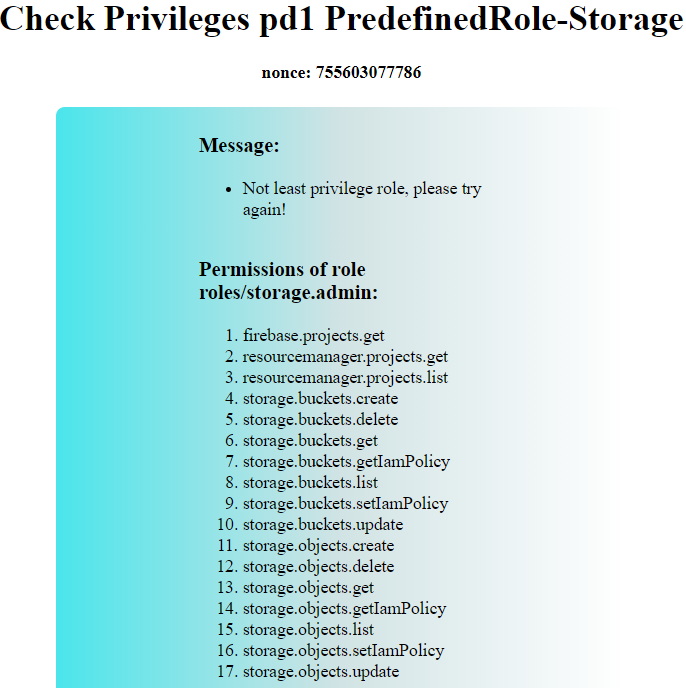
\includegraphics[width=0.5\textwidth]{pic/check}
  \caption {Check Function}
  \label{fig:check}
\end{figure}
To keep players focused on the conceptual tasks and to minimize the amount of time navigating the mechanics of
an exercise, levels each have the same structure and give players a familiar pattern from which to perform the reduction of privileges.
Moreover, the mechanism for solving a level is exactly the mechanism one would perform in an actual project when reducing privileges
on a member through IAM.  Specifically, each level contains two functions, an access function and a check function.
Players begin by visiting the access function which has an over-provisioned set of permissions.

Figure~\ref{fig:access} shows an example of an access function.  The function reveals its source
code and the privileges it has been afforded.  In addition, to support novice players, the CTF provides detailed instructions and links to material 
that can be used to solve the level.  As the figure shows, the access function code requires
permissions to list objects in a bucket, but has been granted a role that has given it additional privileges.  From this, the level
asks the users to visit the service account attached to the access function and change its role to a pre-defined role with least-privileges.
The access function contains a link to a check function that players can then visit after changing the role attached to the access function's
service account. The check function lists the current roles and permissions that are attached to the access function and
displays whether or not it has been set with least privileges. Figure~\ref{fig:check} shows the corresponding output of the check function
for the access function shown previously.  As the figure shows, the pre-defined role
that is currently assigned is {\tt roles/storage.admin} and the check function fails since it is still over-provisioned for what the
access function requires.

\begin{figure}[!h]
  \centering
  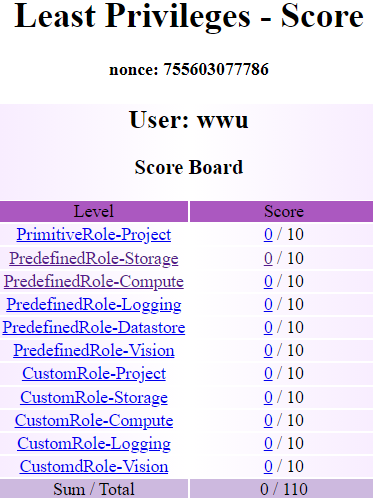
\includegraphics[width=0.4\textwidth]{pic/score}
  \caption {Scoreboard Function}
  \label{fig:score}
\end{figure}

Similar to Jeopardy-style CTF exercises, the Least Privilege CTF also
provides a summary scoreboard for the user to see which levels have been solved in order to allow them to track their progress easily
and get immediate feedback on solutions.  Figure~\ref{fig:score} shows 
the scoreboard interface.  To make it easier for players to focus on the specific goal of each level, the type of role and the service that a level
targets are included in the level name and joined by a dash (first column of Figure~\ref{fig:score}). 

\subsubsection{Deployment ease}
Due to the fact that it is attempting to teach security issues in the cloud,
the Least Privilege CTF assumes players have access to a cloud project that they can use to run
the exercise.  Most public cloud providers support a free-tier that allows one to utilize services without cost and the implementation
of the CTF supports the ability for players to easily deploy and play the CTF at low cost.   Specifically, the CTF features:
\begin{figure}[!h]
  \centering
  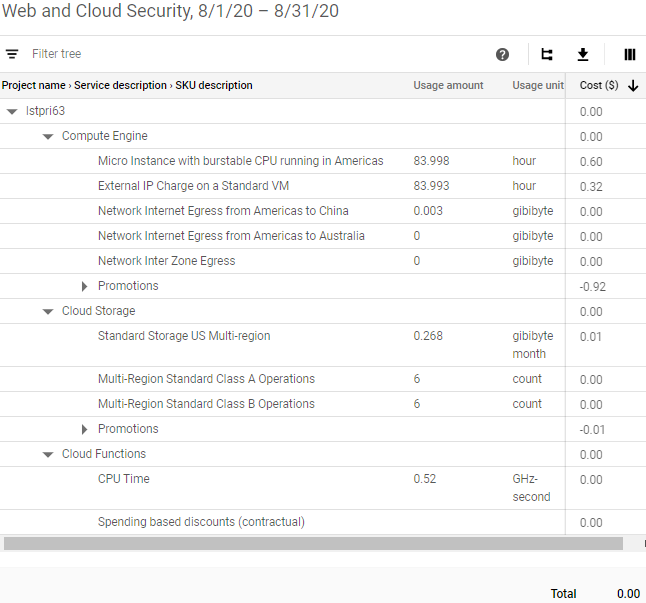
\includegraphics[width=\linewidth]{pic/cost}
  \caption {Billing - Monthly Cost}
  \label{fig:cost}
\end{figure}

\begin{itemize}
  \item {\em Serverless design}: To reduce costs, the CTF is implemented using Cloud Functions, a serverless function platform.  For the CTF, all access and check functions are implemented as Cloud Functions.  There are several advantages in this approach.  First, Cloud Functions require no server management which
  simplifies both development and deployment as one does not have to manage the operational server infrastructure being used.  Second, serverless platforms
  scale the amount of resources deployed based on usage and projects are charged only per function invocation.  As a result, when the CTF is not actively being used, the infrastructure used to handle its functions are brought down and
  the project incurs no charges.  The infrastructure for each function is then instantly spun up upon the player's next access to it.
  With a free tier of 2 million invocations per month for the Cloud Function service~\cite{https://cloud.google.com/free}, this ensures that the exercise
  is free to use.  Third, the use of individual serverless functions for the CTF allows one to easily implement levels since each function can be assigned
  a unique service account with a primitive, pre-defined, or custom role attached to it, naturally aligning it with the conceptual content the CTF is attempting to teach.  The separation also allows levels to be independently developed and provides isolation between them, making it easier to develop additional levels.

  \item {\em Single-command deployment}: Several cloud-based CTFs require individual levels to be brought up and down with explicit commands.  For example, in both Cloud Goat and Thunder CTF, players create and destroy levels individually in order to play them.  In contrast, the Least Privilege CTF deploys its entire set of levels with a single command, allowing players to avoid the mechanics of running the CTF as much as possible.  This is done via the platform's Cloud Deployment
  Manager service, an infrastructure-as-code solution that allows one to programmatically instantiate cloud resources in a consistent and repeatable manner.  Using
  this service, all service accounts, roles, policies, access functions, check functions, and scoreboard functions for the CTF are instantiated all at once using
  a single command and YAML specification file at the beginning of the CTF.  The launching time for the 11 levels currently implemented takes around 4.5 minutes.
  \item {\em Polymorphic level implementation}: When used in courses and certifications, it is desirable for CTFs to be polymorphic in order to ensure unique 
  work has been done in completing it.  The Least Privilege CTF supports polymorphism using the names of the service accounts that the access and check 
  functions are deployed with to support its integration into courses. 
\end{itemize}

\subsubsection{Extensibility}
Least privilege CTF is developed based on Thunder CTF, a scaffolded, scenario-based CTF that helps students learn about and practice cloud security skills on GCP. Each Thunder CTF level includes a yaml development configuration, a python deployment script and an HTML content for hints \cite{Springer}. The modular design and specific structure reduces the process of adding new levels to simply filling in a template. Least privilege CTF inherits the modular structure from Thunder CTF with modification. Rather than deploy each level individually, Least Privileges CTF deploys all required resources specified in the yaml file at one time in parallel with Google Cloud Deployment Manager, which takes about 4.5 mins for 11 levels.

\subsubsection{UI and Cloud Functions}
The type of function to create level instructions and hints in Least Privilege CTF is HTTP function. HTTP functions are invoked by standard HTTP requests and supports common methods like GET, PUT, POST, DELETE and OPTIONS \cite{httpfunc}. A typical procedure in our design framework is that when a function is triggered by events, it waits for responses either returned from a Cloud service or submitted in front-end using POST or GET method. Thanks to the TLS certificates that automatically provisioned in Cloud Functions service, all HTTP functions can be invoked with a secure connection. 

In order to call a function and pass parameters, an URL known as HTTP-Triggered-Endpoint is obtained after each function deployment. Figure~\ref{fig:endpoints} shows the function endpoints printed in Cloud Console shell when deployment manager completes the operation and creates initial levels. In Least Privilege CTF, functions are written in python and interact with other cloud services through APIs. The returned results of a function will be rendered into HTML through Jinja and appear in the form of a web page. Players can access the page in web browser via related function endpoint.

\begin{figure*}[h]
  \centering
  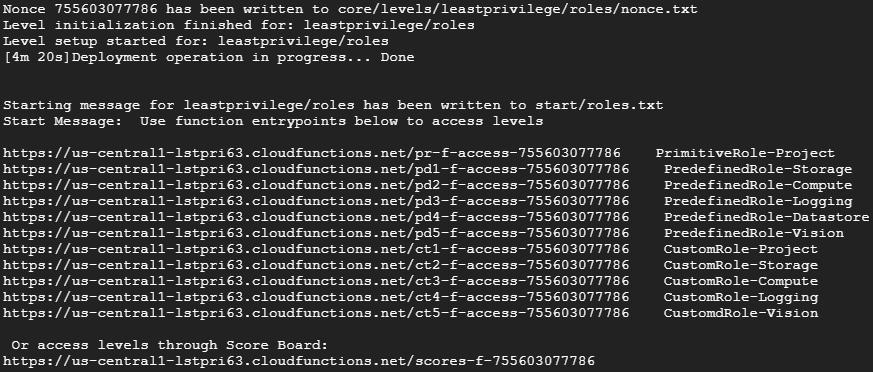
\includegraphics[width=0.7\textwidth]{pic/endpoints}
  \caption {Endpoints}
   \label{fig:endpoints}
\end{figure*}
%%\begin{figure*}[t]
%%  \centering
 %% \begin{tabular}{c}
 %% 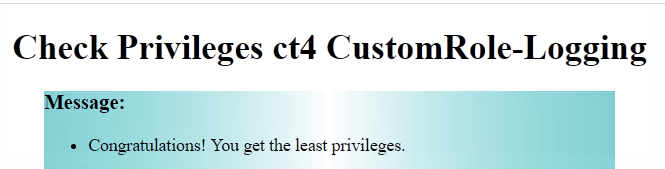
\includegraphics[width=0.60\textwidth]{success}
%%  \end{tabular}
%%\caption{Figure 1: function-validate answer and provide hints}
%%\label{fig:hints}
%%\end{figure*}
